% !TEX encoding = UTF-8 Unicode 
% !TEX root = praca.tex

\chapter*{Badania}

W ninjejszym rozdziale przedstawimy wyniki badań mających na celu porównanie różnych metod XAI stosowanych do wyjaśniania decyzji modeli głębokiego uczenia w kontekście klasyfikacji obrazów.
W badaniach wykozystano LIME, SHAP oraz GradCAM, aby zrozumieć, w jaki sposób te techniki różnią się pod względem generowanych wyjaśnień, dokładności oraz interpretowalności.

Analiza porównawcza została przeprowadzona w oparciu o kilka kluczowych kryteriów:
\begin{itemize}
	\item Średnia redukcja pewności
	\item Średni procentowy wzrost pewności
	\item IoU
\end{itemize}
Podczas badań każdy z powyższych kryteriów został dokładnie oceniony i zanalizowany, aby uzyskać pełny obraz mocnych i słabych stron poszczególnych metod XAI.
Przedstawione wyniki mają na celu dostarczenie wwglądu w to, jak różne techniki wyjaśniania modeli mogą być stosowane w praktyce raz jak wybrać odpowiednią metodę w zależności od konkretnych wymagań aplikacji.


\begin{figure}[h]
	\centering
	\begin{subfigure}[b]{0.3\textwidth}
		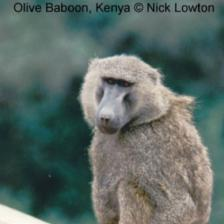
\includegraphics[width=.9\textwidth]{img/examples/appendix/n02486410_08484}
		\caption{Orginalne zdjęcie}  \label{}
	\end{subfigure}
	\begin{subfigure}[b]{0.3\textwidth}
		\centering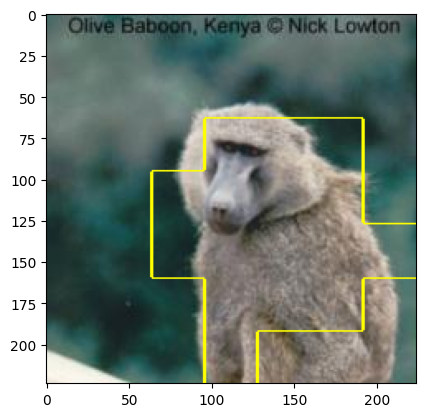
\includegraphics[width=.9\textwidth]{img/examples/appendix/n02486410_08484_gradcam}
		\caption{GradCAM}  \label{}
	\end{subfigure}
	\begin{subfigure}[b]{0.3\textwidth}
		\centering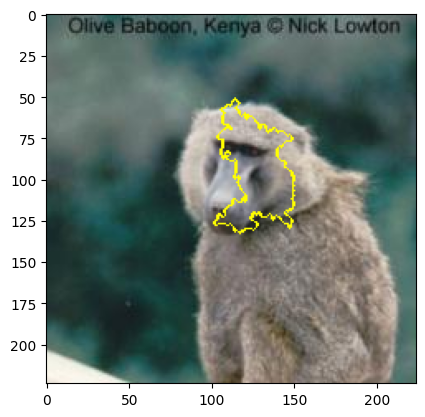
\includegraphics[width=.9\textwidth]{img/examples/appendix/n02486410_08484_lime}
		\caption{LIME}
	\end{subfigure}
	\caption{Przykład spójności wyjaśnień GradCAM i LIME bliskiej średniej - IoU=0.178527}
	\label{}
\end{figure}
\begin{figure}[h]
	\centering
	\begin{subfigure}[b]{0.3\textwidth}
		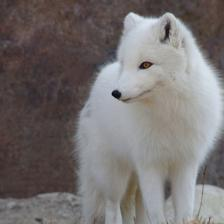
\includegraphics[width=.9\textwidth]{img/examples/appendix/n02120079_49517}
		\caption{Orginalne zdjęcie}  \label{}
	\end{subfigure}
	\begin{subfigure}[b]{0.3\textwidth}
		\centering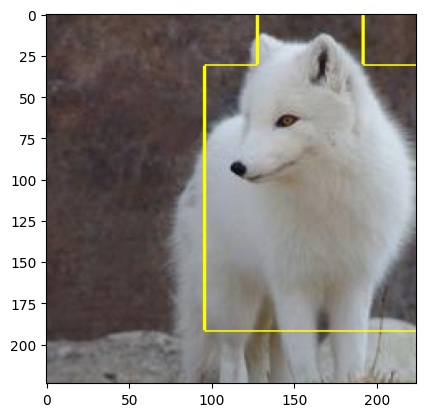
\includegraphics[width=.9\textwidth]{img/examples/appendix/n02120079_49517_gradcam}
		\caption{GradCAM}  \label{}
	\end{subfigure}
	\begin{subfigure}[b]{0.3\textwidth}
		\centering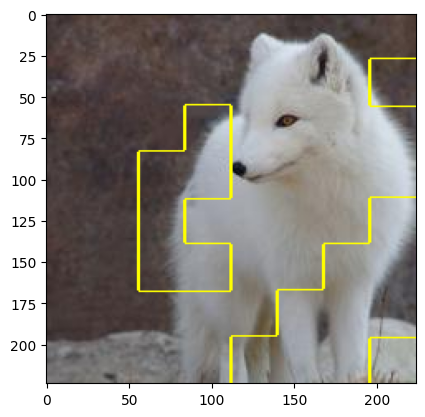
\includegraphics[width=.9\textwidth]{img/examples/appendix/n02120079_49517_shap}
		\caption{SHAP}
	\end{subfigure}
	\caption{Przykład spójności wyjaśnień GradCAM i SHAP bliskiej średniej - IoU=0.111111}
	\label{}
\end{figure}
\begin{figure}[h]
	\centering
	\begin{subfigure}[b]{0.3\textwidth}
		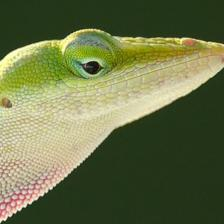
\includegraphics[width=.9\textwidth]{img/examples/appendix/n01682714_14308}
		\caption{Orginalne zdjęcie}  \label{}
	\end{subfigure}
	\begin{subfigure}[b]{0.3\textwidth}
		\centering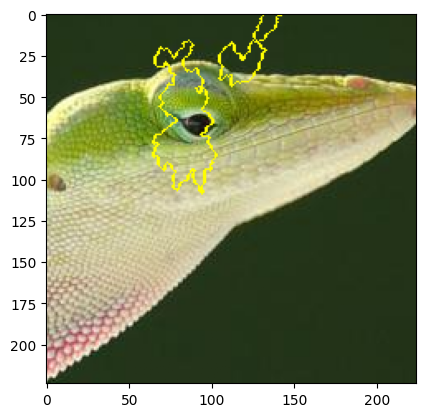
\includegraphics[width=.9\textwidth]{img/examples/appendix/n01682714_14308_lime}
		\caption{LIME}  \label{}
	\end{subfigure}
	\begin{subfigure}[b]{0.3\textwidth}
		\centering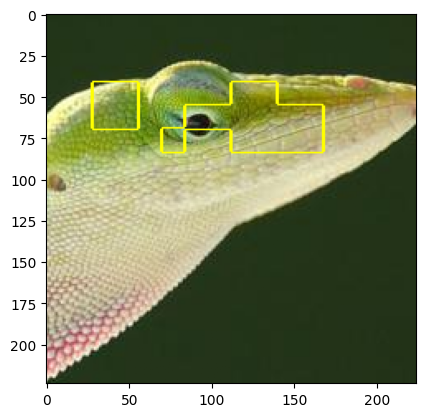
\includegraphics[width=.9\textwidth]{img/examples/appendix/n01682714_14308_shap}
		\caption{SHAP}
	\end{subfigure}
	\caption{Przykład spójności wyjaśnień LIME i SHAP bliskiej średniej - IoU=0.072499}
	\label{}
\end{figure}

\begin{figure}[h]
	\centering
	\begin{subfigure}[b]{0.3\textwidth}
		
\includegraphics[width=.9\textwidth]{img/examples/appendix/n03884397_34878}
		\caption{Orginalne zdjęcie}  \label{}
	\end{subfigure}
	\begin{subfigure}[b]{0.3\textwidth}
		\centering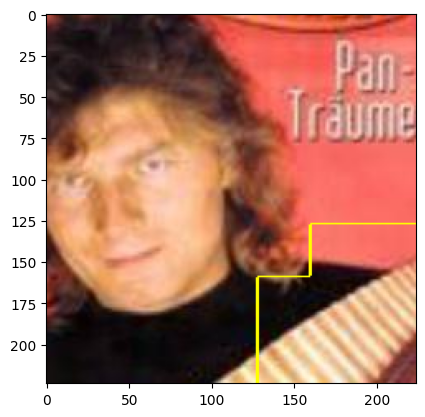
\includegraphics[width=.9\textwidth]{img/examples/appendix/n03884397_34878_gradcam}
		\caption{GradCAM}  \label{}
	\end{subfigure}
	\begin{subfigure}[b]{0.3\textwidth}
		\centering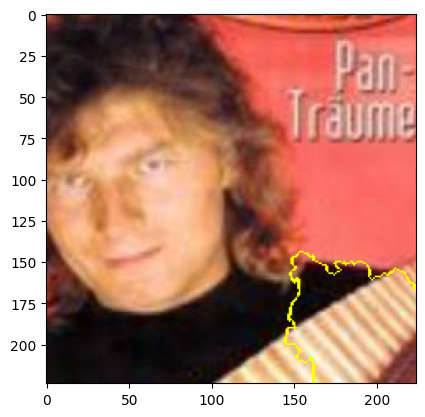
\includegraphics[width=.9\textwidth]{img/examples/appendix/n03884397_34878_lime}
		\caption{LIME}
	\end{subfigure}
	\caption{Przykład spójności wyjaśnień GradCAM i LIME odstające pozytywnie - IoU=0.688791}
	\label{}
\end{figure}
\begin{figure}[h]
	\centering
	\begin{subfigure}[b]{0.3\textwidth}
		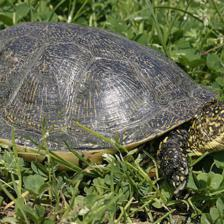
\includegraphics[width=.9\textwidth]{img/examples/appendix/n01667778_32805}
		\caption{Orginalne zdjęcie}  \label{}
	\end{subfigure}
	\begin{subfigure}[b]{0.3\textwidth}
		\centering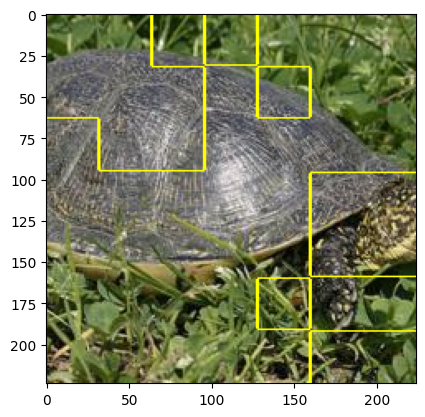
\includegraphics[width=.9\textwidth]{img/examples/appendix/n01667778_32805_gradcam}
		\caption{GradCAM}  \label{}
	\end{subfigure}
	\begin{subfigure}[b]{0.3\textwidth}
		\centering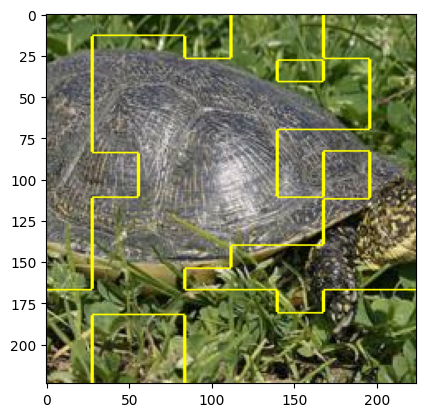
\includegraphics[width=.9\textwidth]{img/examples/appendix/n01667778_32805_shap}
		\caption{SHAP}
	\end{subfigure}
	\caption{Przykład spójności wyjaśnień GradCAM i SHAP odstające pozytywnie - IoU=0.46888}
	\label{}
\end{figure}
\begin{figure}[h]
	\centering
	\begin{subfigure}[b]{0.3\textwidth}
		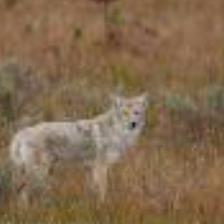
\includegraphics[width=.9\textwidth]{img/examples/appendix/n02114855_39555}
		\caption{Orginalne zdjęcie}  \label{}
	\end{subfigure}
	\begin{subfigure}[b]{0.3\textwidth}
		\centering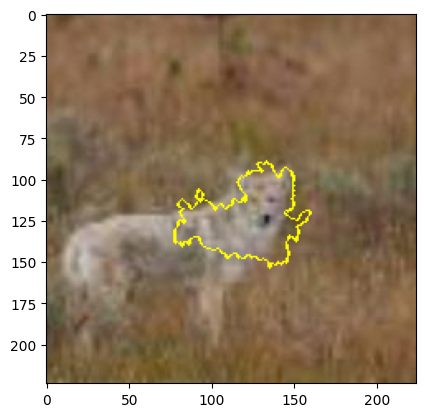
\includegraphics[width=.9\textwidth]{img/examples/appendix/n02114855_39555_lime}
		\caption{LIME}  \label{}
	\end{subfigure}
	\begin{subfigure}[b]{0.3\textwidth}
		\centering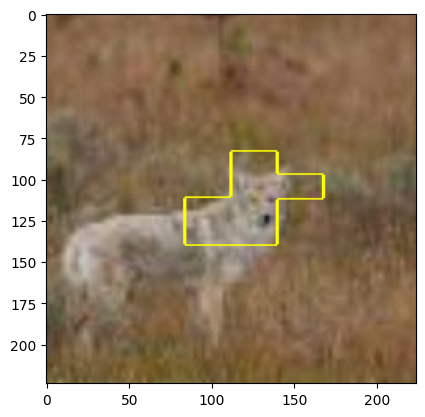
\includegraphics[width=.9\textwidth]{img/examples/appendix/n02114855_39555_shap}
		\caption{SHAP}
	\end{subfigure}
	\caption{Przykład spójności wyjaśnień LIME i SHAP odstające pozytywnie - IoU=0.53489}
	\label{}
\end{figure}

\begin{figure}[h]
	\centering
	\begin{subfigure}[b]{0.3\textwidth}
		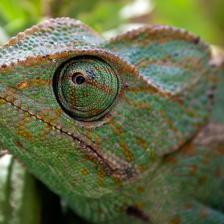
\includegraphics[width=.9\textwidth]{img/examples/appendix/n01694178_23707}
		\caption{Orginalne zdjęcie}  \label{}
	\end{subfigure}
	\begin{subfigure}[b]{0.3\textwidth}
		\centering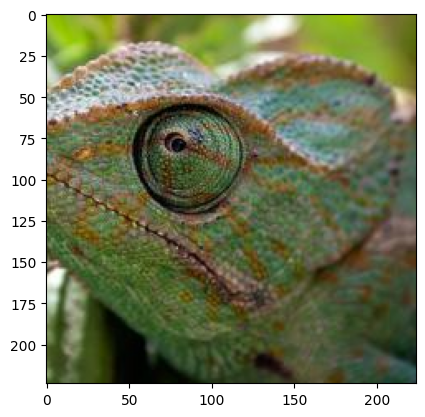
\includegraphics[width=.9\textwidth]{img/examples/appendix/n01694178_23707_gradcam}
		\caption{GradCAM}  \label{}
	\end{subfigure}
	\begin{subfigure}[b]{0.3\textwidth}
		\centering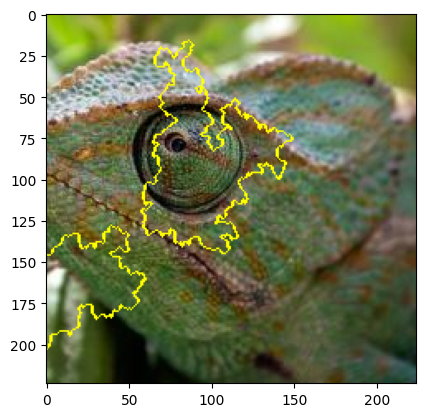
\includegraphics[width=.9\textwidth]{img/examples/appendix/n01694178_23707_lime}
		\caption{LIME}
	\end{subfigure}
	\caption{Przykład spójności wyjaśnień GradCAM i LIME odstające negatywnie - IoU=0.0}
	\label{}
\end{figure}
\begin{figure}[h]
	\centering
	\begin{subfigure}[b]{0.3\textwidth}
		
\includegraphics[width=.9\textwidth]{img/examples/appendix/n01484850_19435}
		\caption{Orginalne zdjęcie}  \label{}
	\end{subfigure}
	\begin{subfigure}[b]{0.3\textwidth}
		\centering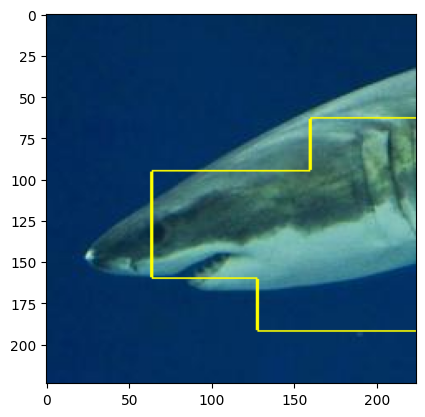
\includegraphics[width=.9\textwidth]{img/examples/appendix/n01484850_19435_gradcam}
		\caption{GradCAM}  \label{}
	\end{subfigure}
	\begin{subfigure}[b]{0.3\textwidth}
		\centering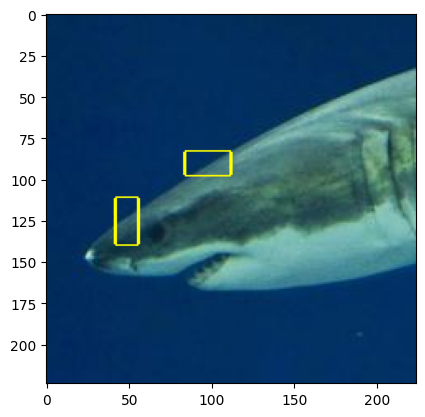
\includegraphics[width=.9\textwidth]{img/examples/appendix/n01484850_19435_shap}
		\caption{SHAP}
	\end{subfigure}
	\caption{Przykład spójności wyjaśnień GradCAM i SHAP  odstające negatywnie- IoU=0.0}
	\label{}
\end{figure}
\begin{figure}[h]
	\centering
	\begin{subfigure}[b]{0.3\textwidth}
		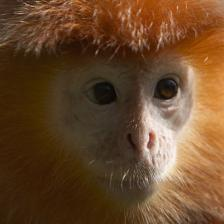
\includegraphics[width=.9\textwidth]{img/examples/appendix/n02488291_05090}
		\caption{Orginalne zdjęcie}  \label{}
	\end{subfigure}
	\begin{subfigure}[b]{0.3\textwidth}
		\centering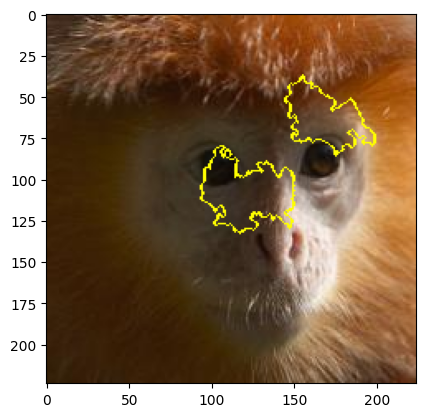
\includegraphics[width=.9\textwidth]{img/examples/appendix/n02488291_05090_lime}
		\caption{LIME}  \label{}
	\end{subfigure}
	\begin{subfigure}[b]{0.3\textwidth}
		\centering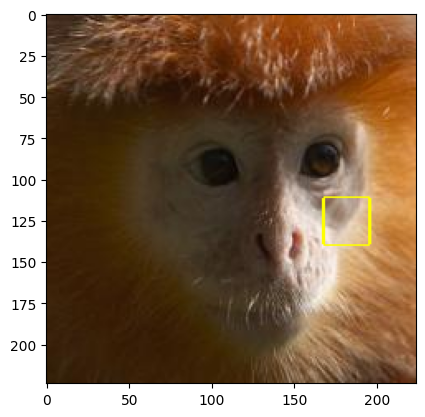
\includegraphics[width=.9\textwidth]{img/examples/appendix/n02488291_05090_shap}
		\caption{SHAP}
	\end{subfigure}
	\caption{Przykład spójności wyjaśnień LIME i SHAP odstające negatywnie - IoU=0.0}
	\label{}
\end{figure}



\section*{Analiza porównacza wyjaśnień}
W tej sekcji przeprowadzono analizę porównawcą wyjaśnień generowanych przez różne metody XAI: LIME, SHAP i GradCAM.
Oceny zostały dokonane na podstawie IoU oraz na podstawie zmiany pewności modelu.
Analiza zostaine przeprowadzona na całym zbiorze danych, a następnie z podziełem na kategorie obrazów oraz w zależności od wielkości obiektów.

Analiza została przeprowadzona na trzech poziomach:
\begin{enumerate}
	\item Na całym zbiorze danych, w celu zrozumienia ogólnej skuteczności każdej z metod XAI.
	\item Z podziałem na kategorie obrazów, w celu zbadania, jak różne typy obiektów wpływają na spójność wyjaśnień.
	\item W zależności od wielkości obiektów na obrazie, aby zbadać, czy rozmiar obiektu ma wpływ na spójność wyjaśnień oraz jakie obszary obrazu są istotne dla różnych metod XAI.
\end{enumerate}

Celem tej analizy było zrozumienie, które metody XAI są najbardziej skuteczne w identyfikacji istotnych cech orazów oraz jakie czynniki mogą wpłynąć na spójność i stabilność wyjaśnień generowanych przez metody.
Dzięki temu możliwe jest lepsze zrozumienie mechanizmów działania każdej z metod i ich potencjalnych zastosowań w praktyce.

\textbf{Analiza na całym zbiorze danych}.
W tej części przeprowadzono analizę porównawczą metod XAI na całym zbiorze danych.
Skupiono się na ocenie Intersection over Union oraz zmianach w pewności modelu po zastosowaniu wyjaśnień.
Celem było zrozumienie, jak skutecznie każda metoda identyfikuje istotne cechy obrazu w kontekście całego zbioru.

\begin{figure}
	\centering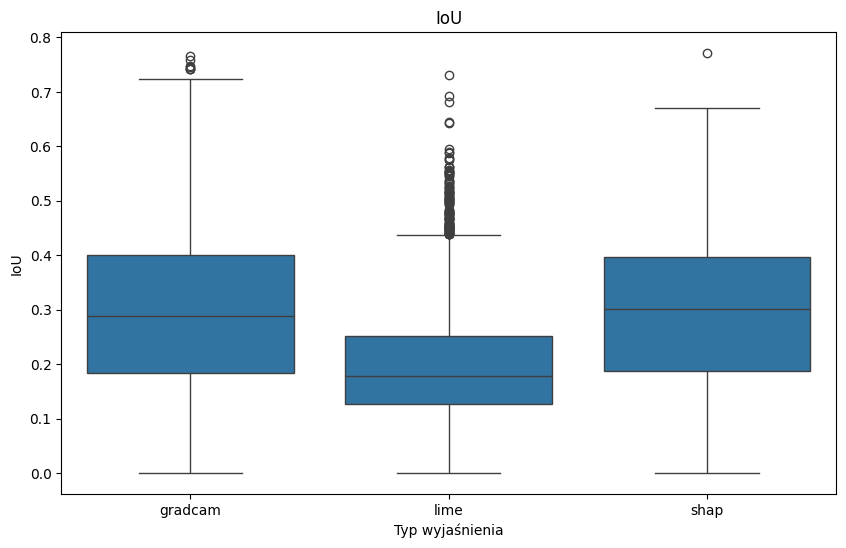
\includegraphics[width=.6\textwidth]{img/base_iou}
	\caption{Wartości IoU  dla stosowanych obrazów}  \label{rys:basiciou}
\end{figure}

\begin{table}
	\centering
	\begin{tabular}{|c|c|c|c|}
		\hline
		\textbf{Metoda XAI}  & GradCAM  & LIME     & SHAP     \\
		\hline
		\textbf{Średnie IoU} & 0.439863 & 0.199370 & 0.292436 \\
		\hline
	\end{tabular}
	\caption{Średnie wartości IoU}
	\label{tab:basiciou}
\end{table}

Wyniki analizy pokazano na wykresie pudełkowym (Rys. \ref{rys:basiciou}), który przedstawia rozkład wartości IoU dla poszczególnych metod XAI.
Dodatkowo, Tabela \ref{tab:basiciou} zawiera średnie wartości IoU dla każdej z metod.

Z wyników wynika, że metoda GradCAM osiągnęła najwyższe średnie wartości IoU, co sugeruje, że generowane przez nią wyjaśnienia najbardziej pokrywają się z rzeczywistymi istotnymi obszarami na obrazach.
Natomiast LIME osiągnęła najniższe średnie IoU.

Te wyniki wskazują, że GradCAM jest najbardziej skuteczny w identyfikacji istotnych cech obrazów na całym zbiorze danych.
Wyższa wartość IoU dla GradCAM może wynikać z doboru niskiego parametru threshold, co powoduje zaznaczenie większego obszaru obrazu.

Metoda LIME, która analizuje lokalne zmiany w predykcji modelu na skutek modyfikacji fragmentów obrazu, wykazała najniższą spójność z rzeczywistymi istotnymi obszarami.
Może to być spowodowane tym, że LIME generuje bardziej szczegółowe, co prowadzi do mniejszej wartości IoU.

Metoda SHAP, która ocenia wpływ każdego piksela na predykcję modelu, uzyskała średnie wartości IoU między GradCAM a LIME, co sugeruje, że generuje wyjaśnienia o umiarkowanej ogólności i precyzji.

% Obszar wyjaśnienia
\begin{figure}
	\centering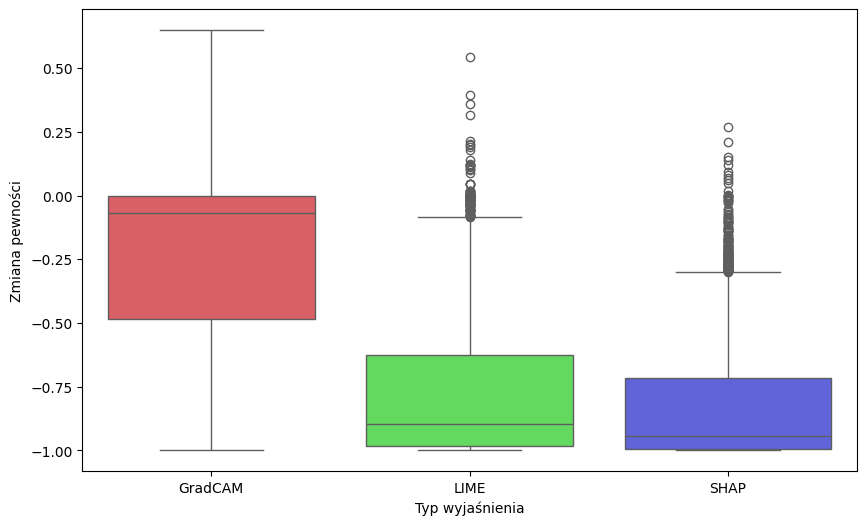
\includegraphics[width=.6\textwidth]{img/base_confidence_exp}
	\caption{Zmiana pewności po pozostawieniu jedynie obszaru wyjaśnienia}  \label{rys:base_confidence_exp}
\end{figure}

\begin{table}
	\centering
	\begin{tabular}{|c|c|c|c|}
		\hline
		\textbf{Metoda XAI}  & GradCAM   & LIME      & SHAP     \\
		\hline
		\textbf{Średnie IoU} & -0.247974 & -0.732920 & -0.58366 \\
		\hline
	\end{tabular}
	\caption{Średni spadek pewności modelu po pozostawieniu jedynie obszaru wyjaśnienia}
	\label{tab:base_confidence_exp}
\end{table}

\begin{table}
	\centering
	\begin{tabular}{|c|c|c|c|}
		\hline
		\textbf{Metoda XAI}  & GradCAM   & LIME     & SHAP     \\
		\hline
		\textbf{Średnie IoU} & 24.8148\% & 2.2222\% & 5.6296\% \\
		\hline
	\end{tabular}
	\caption{Procent przydaków, w których pewność się zwiększyła}
	\label{tab:base_confidence_exp_percent}
\end{table}

Wyniki analizy przedstawiono na wykresie (Rys. \ref{rys:base_confidence_exp}), który ilustruje zmianę pewności modelu po zastosowaniu wyjaśnień.
Tabela \ref{tab:base_confidence_exp} przedstawia średni spadek pewności modelu dla każdej z metod, natomiast Tabela \ref{tab:base_confidence_exp_percent} pokazuje procent przypadków, w których pewność modelu wzrosła po zastosowaniu wyjaśnień.

Metoda GradCAM wykazała najmniejszy spadek pewności modelu, co sugeruje, że wyjaśnienia generowane przez GradCAM są najbardziej zgodne z rzeczywistymi istotnymi obszarami obrazu.
Średni spadek pewności wyniósł -0.247974, a w 24.8148\% przypadków pewność modelu wzrosła, co jest najwyższym wynikiem spośród analizowanych metod.

Metoda LIME, mimo że generuje szczegółowe wyjaśnienia, wykazała największy spadek pewności modelu (-0.732920) i najniższy procent przypadków ze wzrostem pewności (2.2222\%).
Może to sugerować, że LIME identyfikuje obszary, które nie zawsze są kluczowe dla predykcji modelu.

Metoda SHAP, która ocenia wpływ każdego piksela na predykcję, uzyskała średni spadek pewności na poziomie -0.583660 oraz 5.6296\% przypadków ze wzrostem pewności.
Wyniki te wskazują, że SHAP generuje wyjaśnienia o umiarkowanej skuteczności w kontekście identyfikacji istotnych obszarów obrazu.

% Bez obszaru wyjaśnienia
\begin{figure}
	\centering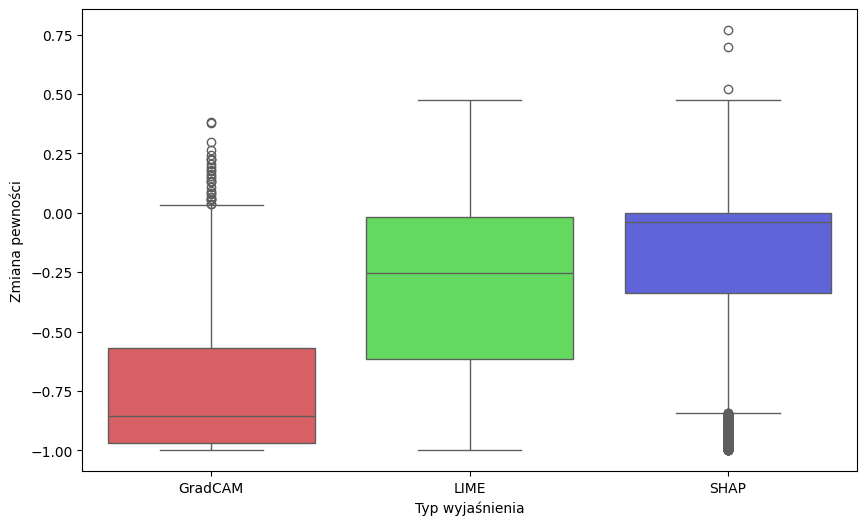
\includegraphics[width=.6\textwidth]{img/base_confidence_no_exp}
	\caption{Zmiana pewności po usunięciu obszaru wyjaśnienia}  \label{rys:base_confidence_no_exp}
\end{figure}

\begin{table}
	\centering
	\begin{tabular}{|c|c|c|c|}
		\hline
		\textbf{Metoda XAI}  & GradCAM   & LIME      & SHAP      \\
		\hline
		\textbf{Średnie IoU} & -0.747604 & -0.404889 & -0.626561 \\
		\hline
	\end{tabular}
	\caption{Średni spadek pewności modelu po usunięciu obszaru wyjaśnienia}
	\label{tab:base_confidence_no_exp}
\end{table}

\begin{table}
	\centering
	\begin{tabular}{|c|c|c|c|}
		\hline
		\textbf{Metoda XAI}  & GradCAM  & LIME     & SHAP     \\
		\hline
		\textbf{Średnie IoU} & 0.9136\% & 6.1728\% & 4.2469\% \\
		\hline
	\end{tabular}
	\caption{Procent przydaków, w których pewność się zwiększyła}
	\label{tab:base_confidence_no_exp_percent}
\end{table}

Wyniki analizy przedstawiono na wykresie (Rys. \ref{rys:base_confidence_no_exp}), który ilustruje zmianę pewności modelu po usunięciu obszaru wyjaśnienia.
Tabela \ref{tab:base_confidence_no_exp} przedstawia średni spadek pewności modelu dla każdej z metod, natomiast Tabela \ref{tab:base_confidence_no_exp_percent} pokazuje procent przypadków, w których pewność modelu wzrosła po usunięciu obszaru wyjaśnienia.

Metoda GradCAM wykazała największy spadek pewności modelu (-0.747604), co sugeruje, że wyjaśnienia generowane przez GradCAM są najbardziej zgodne z rzeczywistymi istotnymi obszarami obrazu.
Niewielki procent przypadków ze wzrostem pewności (0.9136\%) dodatkowo potwierdza, że usunięcie tych obszarów ma znaczący negatywny wpływ na pewność modelu.

Metoda LIME wykazała najmniejszy spadek pewności modelu (-0.404889) oraz najwyższy procent przypadków ze wzrostem pewności (6.1728\%).
Może to sugerować, że LIME identyfikuje obszary, które nie są kluczowe dla predykcji modelu w takim stopniu, jak w przypadku innych metod.

Metoda SHAP uzyskała średni spadek pewności na poziomie -0.626561 oraz 4.2469\% przypadków ze wzrostem pewności.
Wyniki te wskazują, że SHAP generuje wyjaśnienia, które są umiarkowanie skuteczne w kontekście identyfikacji istotnych obszarów obrazu, ale nie są tak trafne jak wyjaśnienia generowane przez GradCAM.

\subsection*{Kategorie}

\textbf{Analiza w zależności od klasy obrazów}.
W tej części dokonamy analizy porównawczej metod XAI z uwzględnieniem różnych kategorii obrazów.
Porównamy skuteczność wyjaśnień generowanych przez LIME, SHAP i GradCAM dla różnych klas.
Celem jest ocena, jak metody radzą sobie w kontekście specyficznych rodzajów obrazów.

\begin{figure}
	\centering
	\begin{subfigure}[b]{0.3\textwidth}
		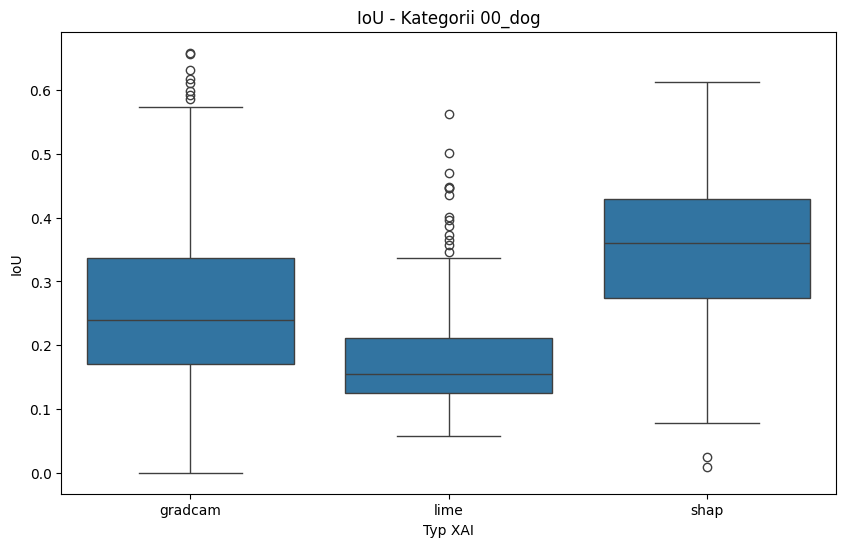
\includegraphics[width=.9\textwidth]{img/base_iou_dog}
		\caption{Dog}  \label{rys:base_iou_dog}
	\end{subfigure}
	\begin{subfigure}[b]{0.3\textwidth}
		\centering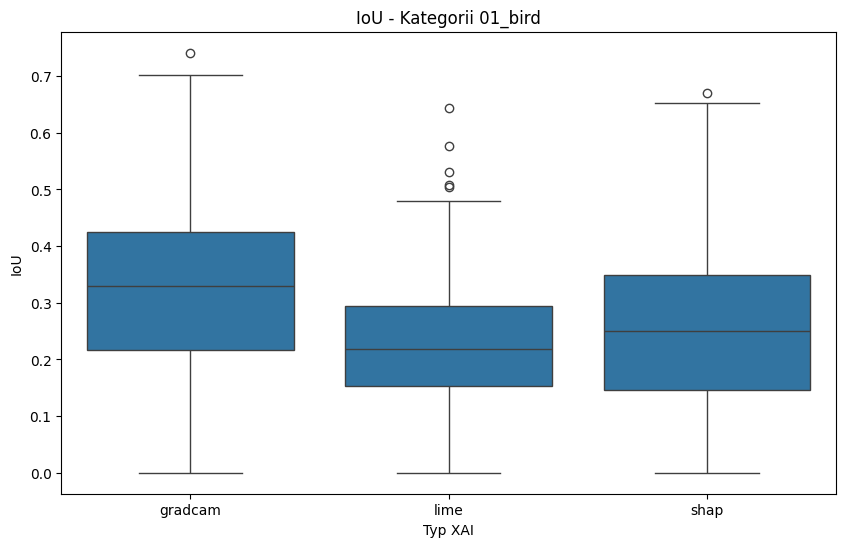
\includegraphics[width=.9\textwidth]{img/base_iou_bird}
		\caption{Bird}  \label{rys:base_iou_bird}
	\end{subfigure}
	\begin{subfigure}[b]{0.3\textwidth}
		\centering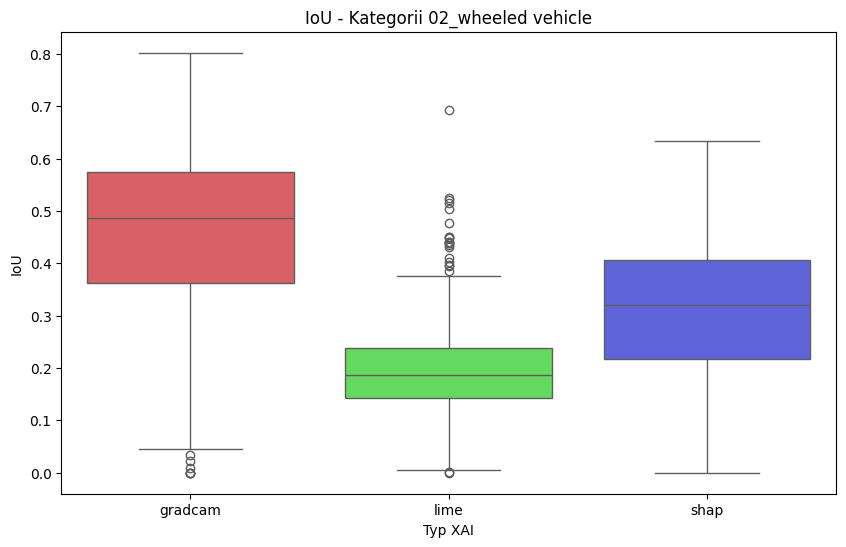
\includegraphics[width=.9\textwidth]{img/base_iou_vehicle}
		\caption{Vehicle}  \label{rys:base_iou_vehicle}
	\end{subfigure}
	\begin{subfigure}[b]{0.3\textwidth}
		\centering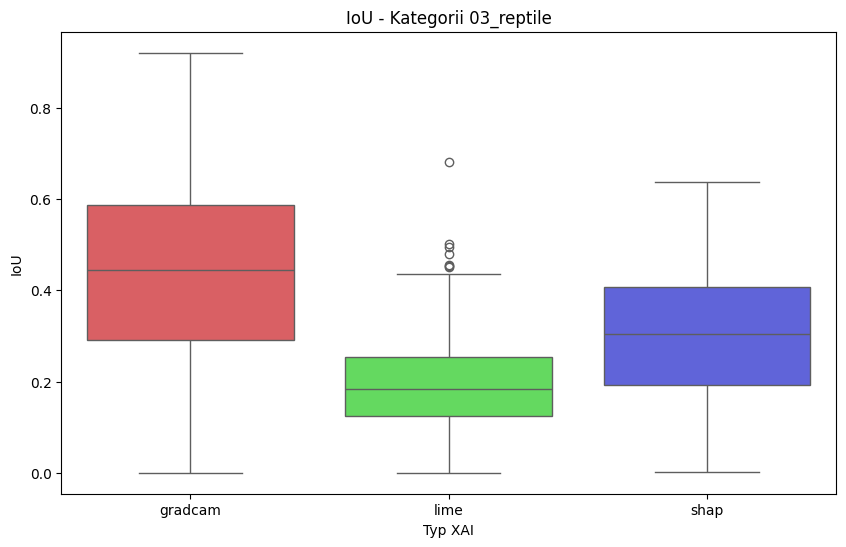
\includegraphics[width=.9\textwidth]{img/base_iou_reptile}
		\caption{Reptile}  \label{rys:base_iou_reptile}
	\end{subfigure}
	\begin{subfigure}[b]{0.3\textwidth}
		\centering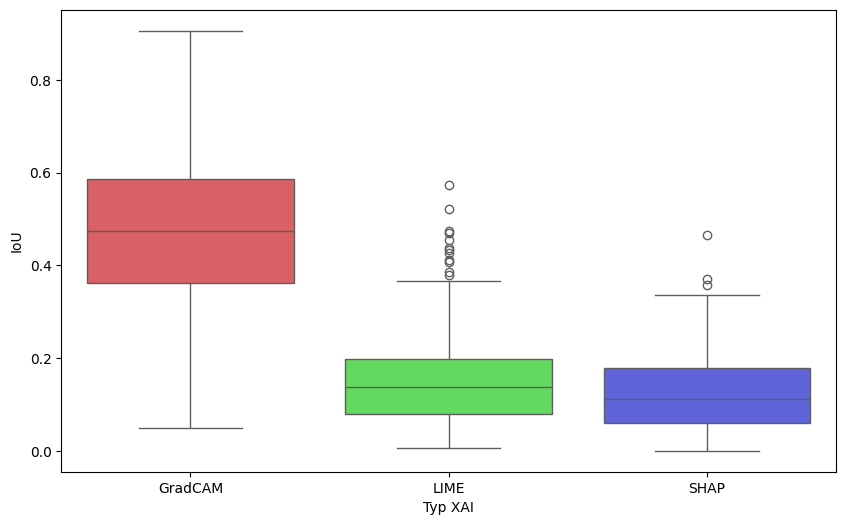
\includegraphics[width=.9\textwidth]{img/base_iou_carnivore}
		\caption{Carnivore}  \label{rys:base_iou_carnivore}
	\end{subfigure}
	\begin{subfigure}[b]{0.3\textwidth}
		\centering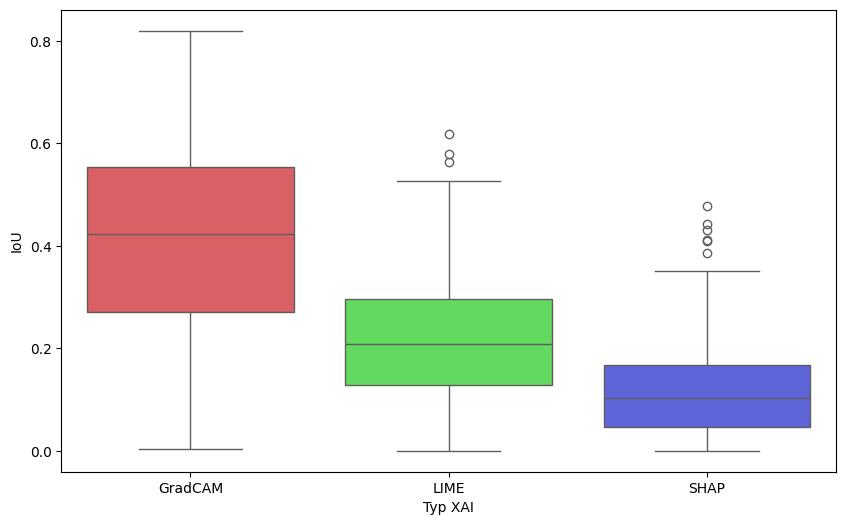
\includegraphics[width=.9\textwidth]{img/base_iou_insect}
		\caption{Insect}  \label{rys:base_iou_insect}
	\end{subfigure}
	\begin{subfigure}[b]{0.3\textwidth}
		\centering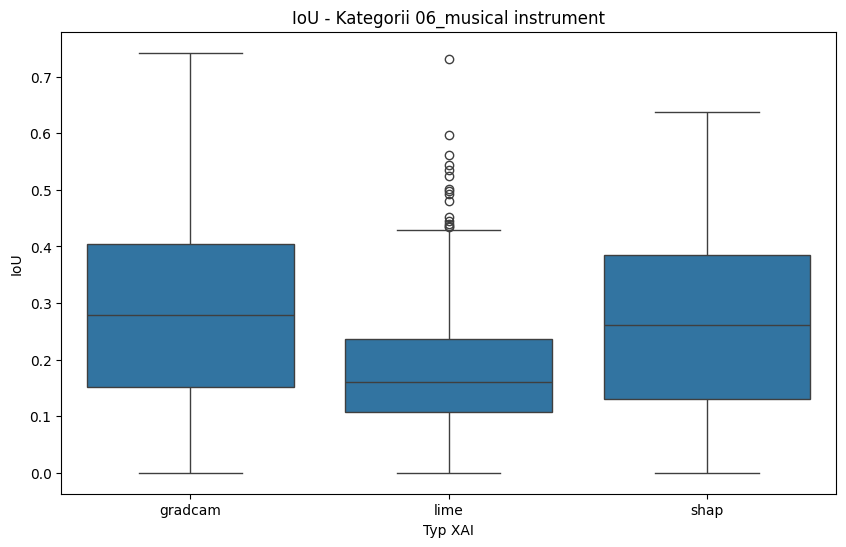
\includegraphics[width=.9\textwidth]{img/base_iou_music}
		\caption{Instrument}  \label{rys:base_iou_music}
	\end{subfigure}
	\begin{subfigure}[b]{0.3\textwidth}
		\centering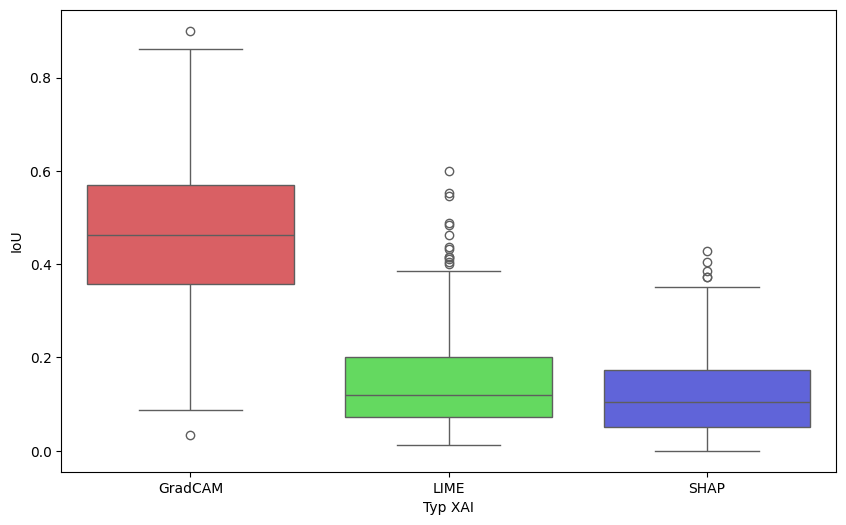
\includegraphics[width=.9\textwidth]{img/base_iou_primate}
		\caption{Primate}  \label{rys:base_iou_primate}
	\end{subfigure}
	\begin{subfigure}[b]{0.3\textwidth}
		\centering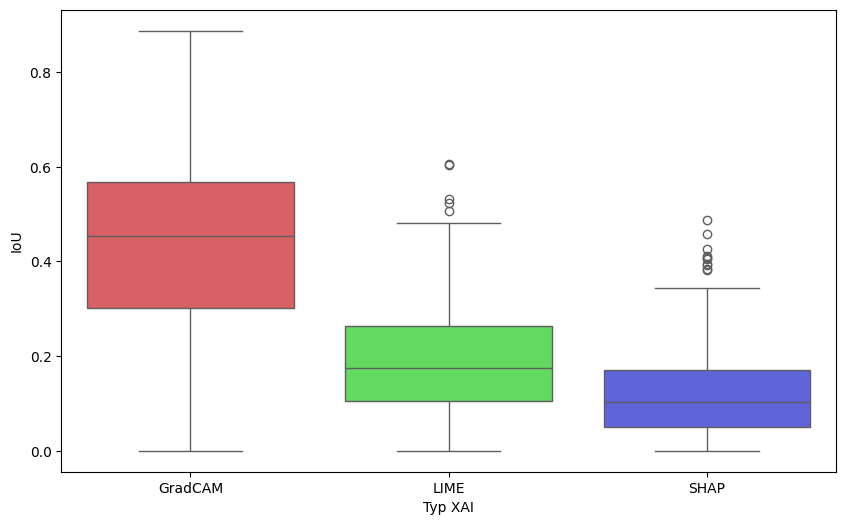
\includegraphics[width=.9\textwidth]{img/base_iou_fish}
		\caption{Fish}  \label{rys:base_iou_fish}
	\end{subfigure}
	\caption{Wartości IoU dla różnych kategorii}
\end{figure}

\begin{table}
	\centering
	\begin{tabular}{|c|c|c|c|}
		\hline
		\textbf{Kategoria}  & \textbf{GradCAM} & \textbf{LIME} & \textbf{SHAP} \\
		\hline
		Pies                & 0.467134         & 0.174455      & 0.351659      \\
		\hline
		Ptak                & 0.428416         & 0.232156      & 0.253825      \\
		\hline
		Pojazd na kołami    & 0.459880         & 0.199560      & 0.308771      \\
		\hline
		Gad                 & 0.436193         & 0.198447      & 0.302146      \\
		\hline
		Mięsożerca          & 0.468916         & 0.173762      & 0.335634      \\
		\hline
		Insekt              & 0.410650         & 0.252195      & 0.255142      \\
		\hline
		Instrument muzyczny & 0.394289         & 0.182606      & 0.261536      \\
		\hline
		Naczelny            & 0.465292         & 0.165912      & 0.332052      \\
		\hline
		Ryba                & 0.427992         & 0.215236      & 0.261161      \\
		\hline
	\end{tabular}
	\caption{IoU dla kategorii}
	\label{tab:base_iou_category}
\end{table}

Wyniki analizy IoU w zależności od kategorii obrazów przedstawiono na wykresach (Rys. \ref{rys:base_iou_dog}-\ref{rys:base_iou_fish}) oraz w Tabeli \ref{tab:base_iou_category}, która zawiera średnie wartości IoU dla poszczególnych metod XAI i kategorii.

Z analizy wynika, że metoda GradCAM osiągnęła najwyższe średnie wartości IoU we wszystkich kategoriach, co wskazuje na jej najwyższą skuteczność w identyfikacji istotnych cech obrazów niezależnie od ich rodzaju.

Metoda SHAP, mimo że generalnie osiągnęła średnie wartości IoU pomiędzy GradCAM a LIME, wykazała szczególną skuteczność w kategoriach Pies (0.351659), Mięsożerca (0.335634) i Naczelny (0.332052), co może sugerować, że SHAP może lepiej radzić sobie z analizą obrazów przedstawiających zwierzęta.

Metoda LIME miała najniższe wartości IoU we wszystkich kategoriach.
Wyniki kategorii Insekt dla LIME (0.252195), były podobne do wyników SHAPA (0.255142), co sugeruje, że w tej konkretnej kategorii obie metody osiągneły porównywalne wyniki.

Ogólnie rzecz biorąc, wyniki te sugerują, że skuteczność metod XAI różni się w zależności od rodzaju obrazów, a wybór odpowiedniej metody powinien uwzględniać specyfikę analizowanej kategorii.

\begin{figure}
	\centering
	\begin{subfigure}[b]{0.3\textwidth}
		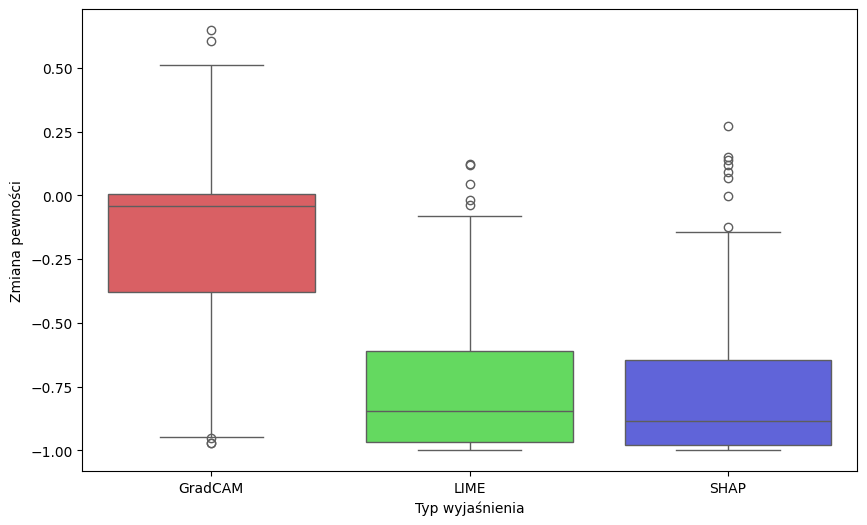
\includegraphics[width=.9\textwidth]{img/base_confidence_exp_dog}
		\caption{Dog}  \label{rys:base_confidence_exp_dog}
	\end{subfigure}
	\begin{subfigure}[b]{0.3\textwidth}
		\centering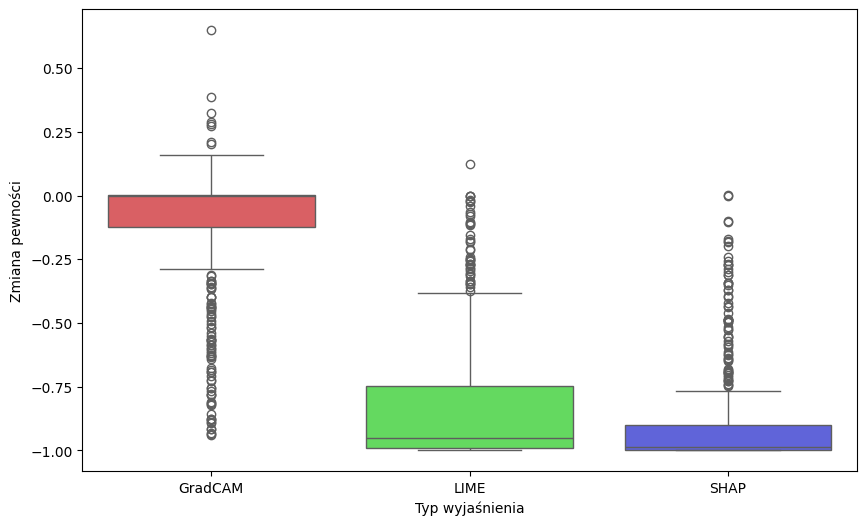
\includegraphics[width=.9\textwidth]{img/base_confidence_exp_bird}
		\caption{Bird}  \label{rys:base_confidence_exp_bird}
	\end{subfigure}
	\begin{subfigure}[b]{0.3\textwidth}
		\centering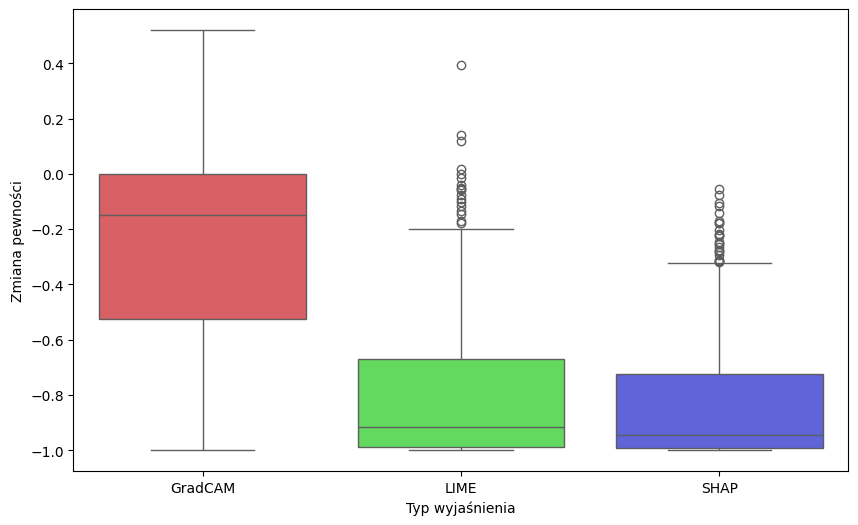
\includegraphics[width=.9\textwidth]{img/base_confidence_exp_vehicle}
		\caption{Vehicle}  \label{rys:base_confidence_exp_vehicle}
	\end{subfigure}
	\begin{subfigure}[b]{0.3\textwidth}
		\centering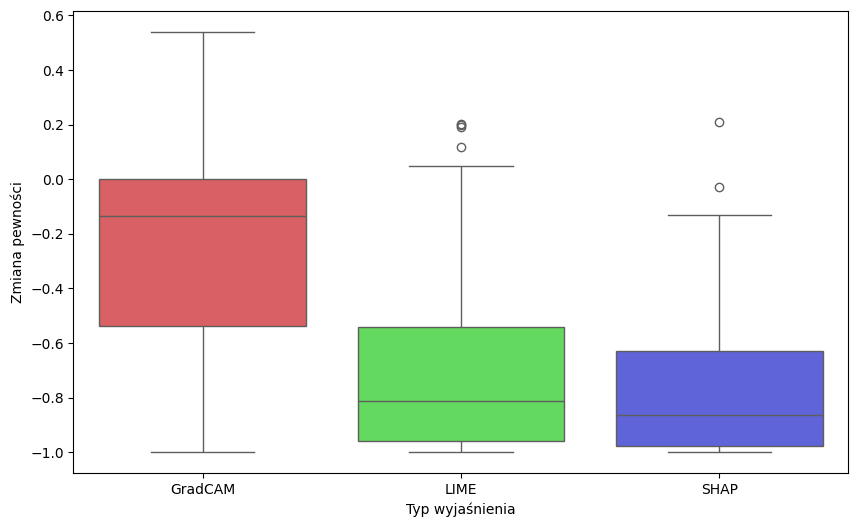
\includegraphics[width=.9\textwidth]{img/base_confidence_exp_reptile}
		\caption{Reptile}  \label{rys:base_confidence_exp_reptile}
	\end{subfigure}
	\begin{subfigure}[b]{0.3\textwidth}
		\centering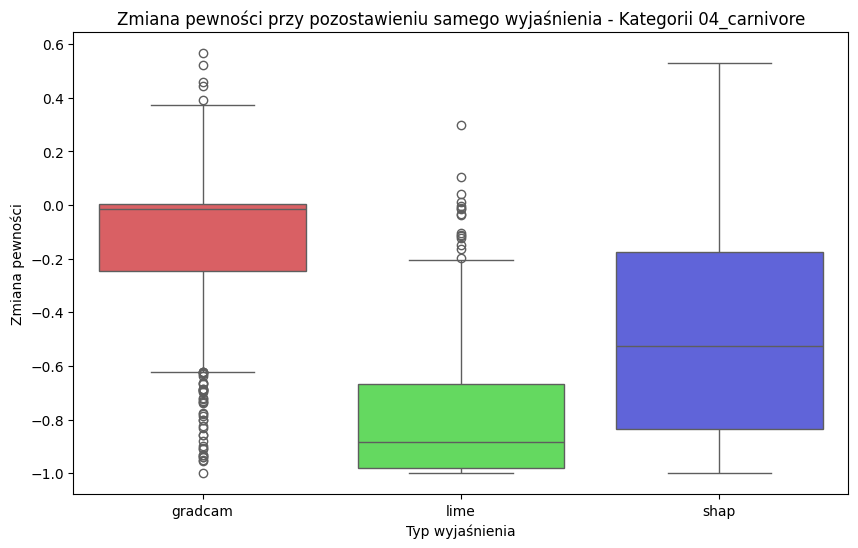
\includegraphics[width=.9\textwidth]{img/base_confidence_exp_carnivore}
		\caption{Carnivore}  \label{rys:base_confidence_exp_carnivore}
	\end{subfigure}
	\begin{subfigure}[b]{0.3\textwidth}
		\centering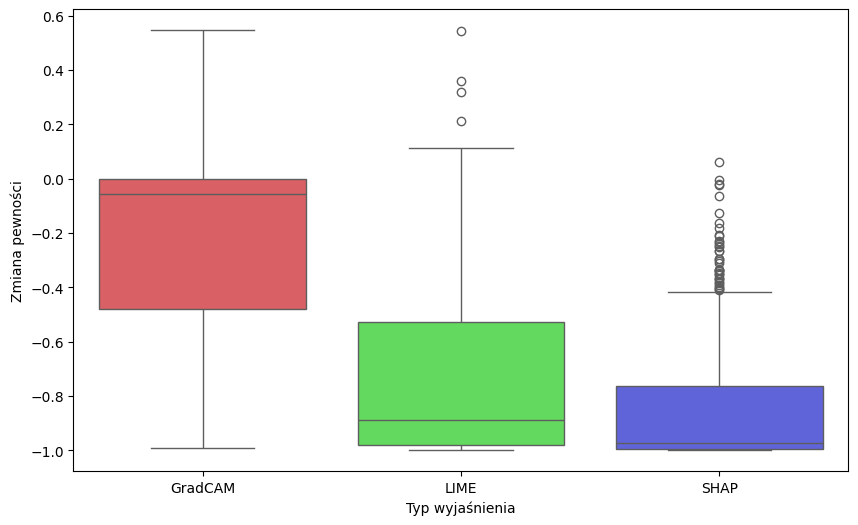
\includegraphics[width=.9\textwidth]{img/base_confidence_exp_insect}
		\caption{Insect}  \label{rys:base_confidence_exp_insect}
	\end{subfigure}
	\begin{subfigure}[b]{0.3\textwidth}
		\centering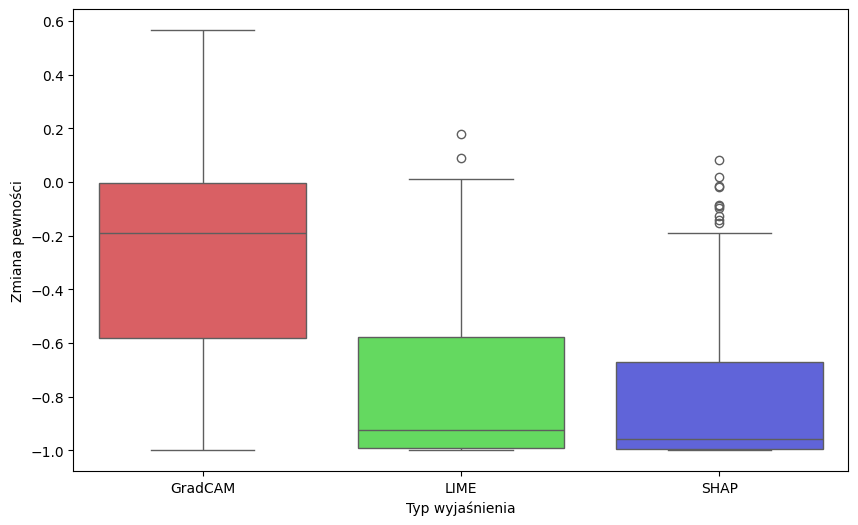
\includegraphics[width=.9\textwidth]{img/base_confidence_exp_music}
		\caption{Instrument}  \label{rys:base_confidence_exp_music}
	\end{subfigure}
	\begin{subfigure}[b]{0.3\textwidth}
		\centering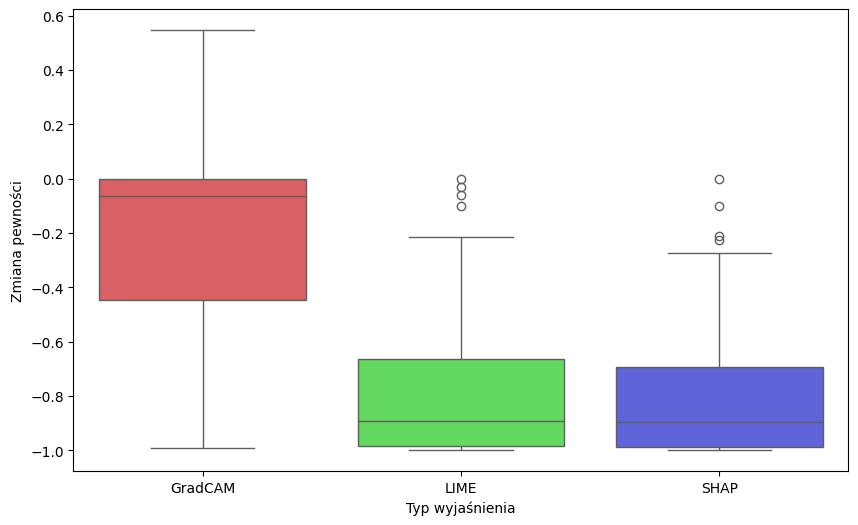
\includegraphics[width=.9\textwidth]{img/base_confidence_exp_primate}
		\caption{Primate}  \label{rys:base_confidence_exp_primate}
	\end{subfigure}
	\begin{subfigure}[b]{0.3\textwidth}
		\centering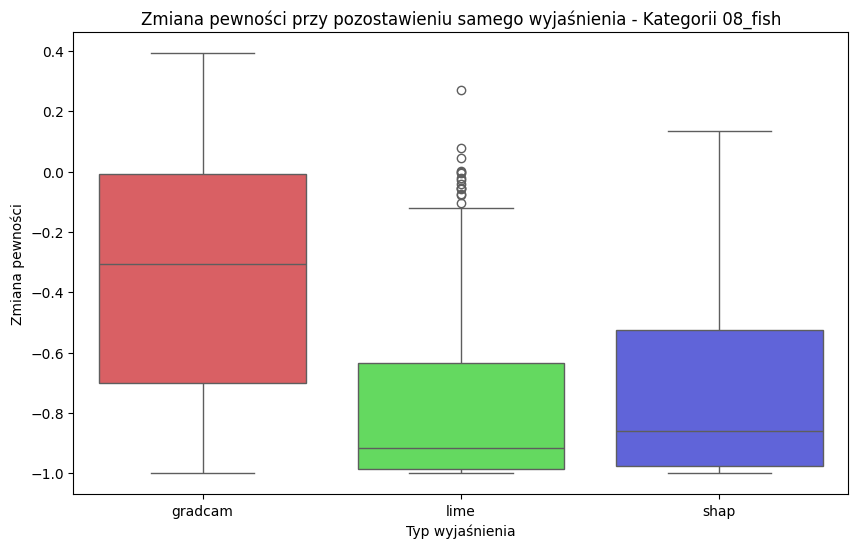
\includegraphics[width=.9\textwidth]{img/base_confidence_exp_fish}
		\caption{Fish}  \label{rys:base_confidence_exp_fish}
	\end{subfigure}
	\caption{Zmiana pewności po pozostawieniu jedynie obszatu wyjaśnienia dla różnych kategorii}
\end{figure}

\begin{table}
	\centering
	\begin{tabular}{|c|c|c|c|}
		\hline
		\textbf{Kategoria}  & \textbf{GradCAM} & \textbf{LIME} & \textbf{SHAP} \\
		\hline
		Pies                & -0.203837        & -0.730913     & -0.523232     \\
		\hline
		Ptak                & -0.126917        & -0.695752     & -0.528825     \\
		\hline
		Pojazd na kołami    & -0.283471        & -0.766767     & -0.626653     \\
		\hline
		Gad                 & -0.281027        & -0.703908     & -0.597428     \\
		\hline
		Mięsożerca          & -0.165199        & -0.781692     & -0.510289     \\
		\hline
		Insekt              & -0.244699        & -0.630861     & -0.594027     \\
		\hline
		Instrument muzyczny & -0.315661        & -0.733294     & -0.602684     \\
		\hline
		Naczelny            & -0.236171        & -0.765780     & -0.557879     \\
		\hline
		Ryba                & -0.374784        & -0.787316     & -0.711981     \\
		\hline
	\end{tabular}
	\caption{Średni spadek pewności modelu po pozostawieniu jedynie obszaru wyjaśnienia dla kategorii}
	\label{tab:category_confidence_exp}
\end{table}

\begin{table}
	\centering
	\begin{tabular}{|c|c|c|c|}
		\hline
		\textbf{Kategoria}  & \textbf{GradCAM} & \textbf{LIME} & \textbf{SHAP} \\
		\hline
		Pies                & 32.8889\%        & 2.2222\%      & 7.1111\%      \\
		\hline
		Ptak                & 35.3333\%        & 4.6667\%      & 6.4444\%      \\
		\hline
		Pojazd na kołami    & 20.0000\%        & 0.4444\%      & 4.4444\%      \\
		\hline
		Gad                 & 25.5556\%        & 1.5556\%      & 6.8889\%      \\
		\hline
		Mięsożerca          & 31.5556\%        & 0.8889\%      & 6.8889\%      \\
		\hline
		Insekt              & 23.1111\%        & 6.2222\%      & 5.1111\%      \\
		\hline
		Instrument muzyczny & 14.8889\%        & 1.7778\%      & 4.4444\%      \\
		\hline
		Naczelny            & 27.3333\%        & 1.3333\%      & 6.2222\%      \\
		\hline
		Ryba                & 12.6667\%        & 0.8889\%      & 3.1111\%      \\
		\hline
	\end{tabular}
	\caption{Procent przypadków, w których pewność się zwiększyła dla kategorii}
	\label{tab:category_confidence_exp_percent}
\end{table}

Wyniki analizy zmiany pewności po pozostawieniu jedynie obszaru wyjaśnienia dla różnych kategorii obrazów przedstawiono na wykresach (Rys. \ref{rys:base_confidence_exp_dog}-\ref{rys:base_confidence_exp_fish}) oraz w Tabelach \ref{tab:category_confidence_exp} i \ref{tab:category_confidence_exp_percent}, które zawierają średni spadek pewności modelu oraz procent przypadków, w których pewność modelu się zwiększyła.

Z analizy wynika, że metoda GradCAM konsekwentnie powoduje najmniejszy spadek pewności modelu w różnych kategoriach obrazów, co wskazuje na jej skuteczność w zachowywaniu kluczowych informacji przy pozostawieniu jedynie obszaru wyjaśnienia.
Najmniejszy spadek pewności odnotowano w kategorii Ptak (-0.126917), a największy w kategorii Ryba (-0.374784).

Metoda SHAP, mimo że generalnie osiągnęła średnie wartości pomiędzy GradCAM a LIME, wykazała mniejsze spadki pewności w kategoriach Pies (-0.523232), Mięsożerca (-0.510289), i Naczelny (-0.557879), co może sugerować, że jest bardziej efektywna w analizie obrazów przedstawiających zwierzęta.

Metoda LIME miała najniższe wartości we wszystkich kategoriach, co wskazuje na największy spadek pewności modelu. Największy spadek pewności zaobserwowano w kategorii Ryba (-0.787316), a najmniejszy w kategorii Ptak (-0.695752).

Dodatkowo, analiza procentu przypadków, w których pewność modelu się zwiększyła, pokazuje, że GradCAM również w tej mierze osiąga lepsze wyniki. W kategorii Ptak aż 35.3333\% przypadków odnotowało wzrost pewności modelu, co jest najwyższą wartością spośród wszystkich metod i kategorii.

Podsumowując, GradCAM wykazuje najwyższą skuteczność w zachowywaniu i podwyższaniu pewności modelu po pozostawieniu jedynie obszaru wyjaśnienia, niezależnie od kategorii obrazu.
SHAP osiąga lepsze wyniki w kategoriach zwierząt, podczas gdy LIME wykazuje największe spadki pewności modelu.

\begin{figure}
	\centering
	\begin{subfigure}[b]{0.3\textwidth}
		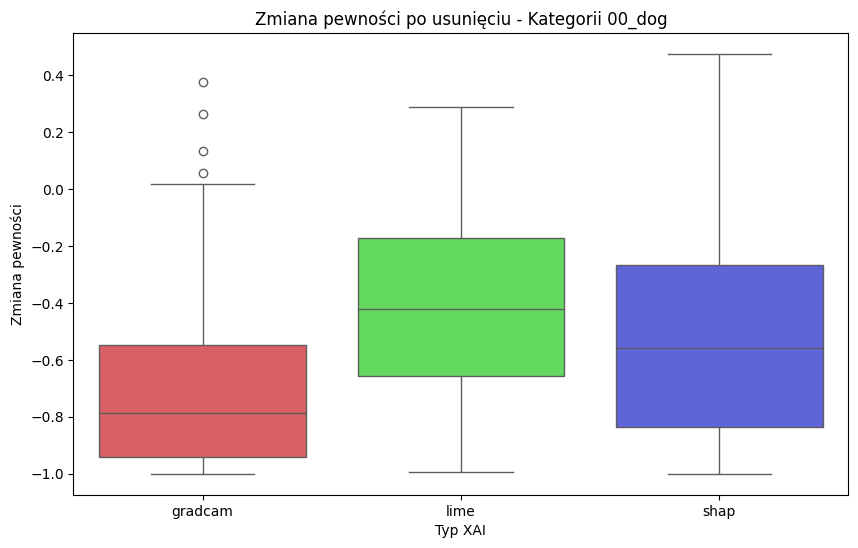
\includegraphics[width=.9\textwidth]{img/base_confidence_no_exp_dog}
		\caption{Dog}  \label{rys:base_confidence_no_exp_dog}
	\end{subfigure}
	\begin{subfigure}[b]{0.3\textwidth}
		\centering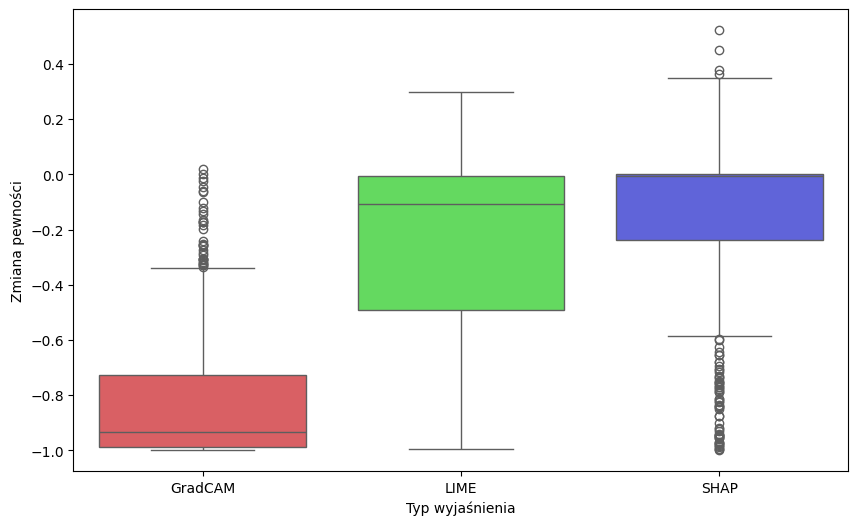
\includegraphics[width=.9\textwidth]{img/base_confidence_no_exp_bird}
		\caption{Bird}  \label{rys:base_confidence_no_exp_bird}
	\end{subfigure}
	\begin{subfigure}[b]{0.3\textwidth}
		\centering\includegraphics[width=.9\textwidth]{img/base_confidence_no_exp_vehicle}
		\caption{Vehicle}  \label{rys:base_confidence_no_exp_vehicle}
	\end{subfigure}
	\begin{subfigure}[b]{0.3\textwidth}
		\centering\includegraphics[width=.9\textwidth]{img/base_confidence_no_exp_reptile}
		\caption{Reptile}  \label{rys:base_confidence_no_exp_reptile}
	\end{subfigure}
	\begin{subfigure}[b]{0.3\textwidth}
		\centering\includegraphics[width=.9\textwidth]{img/base_confidence_no_exp_carnivore}
		\caption{Carnivore}  \label{rys:base_confidence_no_exp_carnivore}
	\end{subfigure}
	\begin{subfigure}[b]{0.3\textwidth}
		\centering\includegraphics[width=.9\textwidth]{img/base_confidence_no_exp_insect}
		\caption{Insect}  \label{rys:base_confidence_no_exp_insect}
	\end{subfigure}
	\begin{subfigure}[b]{0.3\textwidth}
		\centering\includegraphics[width=.9\textwidth]{img/base_confidence_no_exp_music}
		\caption{Instrument}  \label{rys:base_confidence_no_exp_music}
	\end{subfigure}
	\begin{subfigure}[b]{0.3\textwidth}
		\centering\includegraphics[width=.9\textwidth]{img/base_confidence_no_exp_primate}
		\caption{Primate}  \label{rys:base_confidence_no_exp_primate}
	\end{subfigure}
	\begin{subfigure}[b]{0.3\textwidth}
		\centering\includegraphics[width=.9\textwidth]{img/base_confidence_no_exp_fish}
		\caption{Fish}  \label{rys:base_confidence_no_exp_fish}
	\end{subfigure}
	\caption{Zmiana pewności po usunięciu obszaru wyjaśnienia dla różnych kategorii}
\end{figure}

\begin{table}
	\centering
	\begin{tabular}{|c|c|c|c|}
		\hline
		\textbf{Kategoria}  & \textbf{GradCAM} & \textbf{LIME} & \textbf{SHAP} \\
		\hline
		Pies                & -0.712184        & -0.417865     & -0.537021     \\
		\hline
		Ptak                & -0.815407        & -0.434966     & -0.675336     \\
		\hline
		Pojazd na kołami    & -0.731519        & -0.413569     & -0.622449     \\
		\hline
		Gad                 & -0.709709        & -0.368300     & -0.614917     \\
		\hline
		Mięsożerca          & -0.709833        & -0.316740     & -0.542409     \\
		\hline
		Insekt              & -0.802191        & -0.421774     & -0.676712     \\
		\hline
		Instrument muzyczny & -0.729714        & -0.423949     & -0.627190     \\
		\hline
		Naczelny            & -0.730957        & -0.368148     & -0.621441     \\
		\hline
		Ryba                & -0.786923        & -0.478694     & -0.721575     \\
		\hline
	\end{tabular}
	\caption{Średni spadek pewności modelu po usunięciu obszaru wyjaśnienia dla kategorii}
	\label{tab:category_confidence_no_exp}
\end{table}

Wyniki analizy zmiany pewności po usunięciu obszaru wyjaśnień dla różnych kategorii obrazów przedstawiono na wykresach (Rys. \ref{rys:base_confidence_no_exp_dog}-\ref{rys:base_confidence_no_exp_fish}) oraz w Tabelach \ref{tab:category_confidence_no_exp}, które zawierają średni spadek pewności modelu.

Z analizy wynika, że metoda LIME powoduje najmniejszy spadek pewności modelu po usunięciu obszaru wyjaśnienia w większości kategorii obrazów, co sugeruje, że generowane przez nią wyjaśnienia są mniej istotne dla decyzji modelu.
Najmniejszy spadek pewności odnotowano w kategorii Mięsożerca (-0.316740), a największy w kategorii Ptak (-0.434966).

Metoda SHAP wykazuje średnie wartości spadku pewności pomiędzy LIME a GradCAM.
Warto zauważyć, że najmniejszy spadek pewności modelu po usunięciu obszaru wyjaśnienia dla SHAP wystąpił w kategorii Mięsożerca (-0.542409), co może sugerować, że SHAP jest bardziej skuteczny w analizie obrazów przedstawiających zwierzęta.

Metoda GradCAM wykazuje największe spadki pewności modelu po usunięciu obszaru wyjaśnienia we wszystkich kategoriach obrazów.
Największy spadek pewności odnotowano w kategorii Ptak (-0.815407), co wskazuje na to, że obszary wyjaśnień generowanych przez GradCAM są kluczowe dla decyzji modelu w przypadku obrazów tej kategorii.

Podsumowując, LIME powoduje najmniejszy spadek pewności modelu po usunięciu obszaru wyjaśnienia, co sugeruje, że generowane przez nią wyjaśnienia są mniej istotne dla decyzji modelu.
Metoda SHAP osiąga średnie wyniki pomiędzy LIME a GradCAM, a GradCAM wykazuje największe spadki pewności modelu, co sugeruje, że obszary wyjaśnień generowanych przez tę metodę są kluczowe dla decyzji modelu.

\subsection*{Wielkość obiektu}

\textbf{Analiza w zależności od wielkości obiektu}.
Przeanalizowano, jak metody XAI radziły sobie w identyfikacji istotnych cech obrazów w zależności od wielkości obiektów.
Porównamy wyniki IoU oraz zmiany pewności modelu dla małych, średnich oraz dużych obiektów.
Celem było zrozumienie, jak wielkość obiektu wpływa na skuteczność wyjaśnień generowanych przez różne metody.

\textbf{IoU}
\begin{figure}
	\centering
	\begin{subfigure}[b]{0.3\textwidth}
		\centering\includegraphics[width=.9\textwidth]{img/size_iou_gradcam}
		\caption{GradCAM}  \label{rys:size_iou_gradcam}
	\end{subfigure}
	\begin{subfigure}[b]{0.3\textwidth}
		\centering\includegraphics[width=.9\textwidth]{img/size_iou_lime}
		\caption{LIME}  \label{rys:size_iou_lime}
	\end{subfigure}
	\begin{subfigure}[b]{0.3\textwidth}
		\centering\includegraphics[width=.9\textwidth]{img/size_iou_shap}
		\caption{SHAP}  \label{rys:size_iou_shap}
	\end{subfigure}
	\caption{Wartości IoU w zależności od rozmiaru obiektu na obrazie}
\end{figure}

\begin{table}
	\centering
	\begin{tabular}{|c|c|c|c|}
		\hline
		\textbf{Kategoria} & \textbf{GradCAM} & \textbf{LIME} & \textbf{SHAP} \\
		\hline
		S                  & 0.345227         & 0.276572      & 0.171397      \\
		\hline
		M                  & 0.477717         & 0.186679      & 0.314621      \\
		\hline
		L                  & 0.497586         & 0.131633      & 0.396037      \\
		\hline
	\end{tabular}
	\caption{Średnie wartości IoU w zależności od rozmiaru obiektu na obrazie}
	\label{tab:size_iou}
\end{table}

Wyniki analizy IoU dla różnych wielkości obiektów obrazów przedstawiono na wykresach (Rys. \ref{rys:size_iou_gradcam}-\ref{rys:size_iou_shap}) oraz w Tabeli \ref{tab:size_iou}, która zawiera średnie wartości IoU.

GradCAM osiągnął najlepsze wyniki IoU dla dużych obiektów.
Skuteczność GradCAM jest proporcjonalna do wielkości obiektu: im większy obiekt, tym wyższa wartość IoU.
Wskazuje to, że GradCAM lepiej identyfikuje kluczowe obszary na obrazach zawierające większe obiekty.
Może to być spowodowane niską rozdzielczością wyjaśnień wynikającą z wielkości ostatniej warstwy konwolucyjnej w ResNet50.

LIME osiągnął najniższą wartość IoU dla dużych obiektów.
Skuteczność LIME jest odwrotnie proporcjonalna do wielkości obiektu:  im większy obiekt, tym niższa wartość IoU.
Wskazuje to, że LIME lepiej radzi sobie z mniejszymi obiektami, mając trudności z identyfikacją kluczowych cech na większych obiektach.
Może to być spowodowane ustawionymi parametrami, gdyż LIME jest wysoce wrażliwy na parametry.

SHAP osiągał najlepsze wyniki dla dużych obiektów.
Skuteczność SHAP również była proporcjonalna do wielkości obiektu: im większy obiekt tym wyższa wartość IoU.
Podobnie jak GradCAM, SHAP lepiej identyfikuje istotne obszary dla większych obiektów, choć jego skuteczność nie jest tak wysoka jak dla GradCAM.

\textbf{Zmiana pewności przy pozostawieniu samego wyjaśnienia}
\begin{figure}
	\centering
	\begin{subfigure}[b]{0.3\textwidth}
		\centering\includegraphics[width=.9\textwidth]{img/size_confidence_exp_gradcam}
		\caption{GradCAM}  \label{rys:size_confidence_mask_gradcam}
	\end{subfigure}
	\begin{subfigure}[b]{0.3\textwidth}
		\centering\includegraphics[width=.9\textwidth]{img/size_confidence_exp_lime}
		\caption{LIME}  \label{rys:size_confidence_mask_lime}
	\end{subfigure}
	\begin{subfigure}[b]{0.3\textwidth}
		\centering\includegraphics[width=.9\textwidth]{img/size_confidence_exp_shap}
		\caption{SHAP}  \label{rys:size_confidence_mask_shap}
	\end{subfigure}
	\caption{Zmiana pewności przy usunięciu obszarów wyjaśnienia}
\end{figure}

\begin{table}
	\centering
	\begin{tabular}{|c|c|c|c|}
		\hline
		\textbf{Kategoria} & \textbf{GradCAM} & \textbf{LIME} & \textbf{SHAP} \\
		\hline
		S                  & -0.262645        & -0.658282     & -0.567562     \\
		\hline
		M                  & -0.242182        & -0.753241     & -0.592994     \\
		\hline
		L                  & -0.238938        & -0.789269     & -0.590214     \\
		\hline
	\end{tabular}
	\caption{Zmiana pewności przy samym obszarze wyjaśnienia}
	\label{tab:size_confidence_exp}
\end{table}

\begin{table}
	\centering
	\begin{tabular}{|c|c|c|c|}
		\hline
		\textbf{Kategoria} & \textbf{GradCAM} & \textbf{LIME} & \textbf{SHAP} \\
		\hline
		S                  & 22.7171\%        & 4.0831\%      & 6.6815\%      \\
		\hline
		M                  & 26.3048\%        & 1.6701\%      & 5.5672\%      \\
		\hline
		L                  & 25.3555\%        & 0.8689\%      & 4.5814\%      \\

		\hline
	\end{tabular}
	\caption{Procent przypadków, w których pewność się zwiększyła sam obszar wyjaśnienia dla rozmirów}
	\label{tab:size_confidence_exp_percent}
\end{table}

Wyniki analizy zmiany pewności po pozostawieniu jedynie obszarów wyjaśnienia dla różnych wielkości obiektów obrazów przedstawiono na wykresach (Rys. \ref{rys:size_confidence_mask_gradcam}-\ref{rys:size_confidence_mask_shap}) oraz w Tabelach \ref{tab:size_confidence_exp} oraz \ref{tab:size_confidence_exp_percent}.

Zmiana pewności modelu po pozostawieniu obszarów wyjaśnień jest najmniejsza dla dużych obiektów.
Spadek pewności jest mniejszy dla większych obiektów, co może sugerować, że GradCAM skuteczniej identyfikuje kluczowe obszary dla większych obiektów, które mają większy wpływ na pewność modelu.
GradCAM osiągnął najwyższy procent przypadków, w których pewność się zwiększyła dla średnich obiektów.
GradCAM wykazuje największą skuteczność dla średnich obiektów w kontekście zwiększania pewności modelu, chociaż różnice pomiędzy kategoriami rozmiarów nie są znaczne.

LIME wykazał największy spadek pewności dla dużych obiektów.
Spadek pewności jest większy dla większych obiektów, co może sugerować, że LIME ma trudności z identyfikacją kluczowych obszarów dla większych obiektów, co skutkuje większym spadkiem pewności modelu.
LIME osiągnął największy procent przypadków, w których pewność się zwiększyła dla małych obiektów.
LIME wykazuje największą skuteczność dla małych obiektów w kontekście zwiększania pewności modelu, co potwierdza jego lepszą zdolność do pracy z mniejszymi obiektami.

SHAP wykazał najmniejszy spadek pewności dla dużych obiektów.
Spadek pewności jest stosunkowo podobny dla wszystkich rozmiarów obiektów, z niewielką tendencją do mniejszego spadku dla większych obiektów, co może sugerować, że SHAP jest bardziej stabilny w identyfikacji kluczowych obszarów niezależnie od wielkości obiektu.

\textbf{Zmiana pewności po usunięciu obszarów wyjaśnień}
\begin{figure}
	\centering
	\begin{subfigure}[b]{0.3\textwidth}
		\centering\includegraphics[width=.9\textwidth]{img/size_confidence_no_exp_gradcam}
		\caption{GradCAM}  \label{rys:size_confidence_no_exp_gradcam}
	\end{subfigure}
	\begin{subfigure}[b]{0.3\textwidth}
		\centering\includegraphics[width=.9\textwidth]{img/size_confidence_no_exp_lime}
		\caption{LIME}  \label{rys:size_confidence_no_exp_lime}
	\end{subfigure}
	\begin{subfigure}[b]{0.3\textwidth}
		\centering\includegraphics[width=.9\textwidth]{img/size_confidence_no_exp_shap}
		\caption{SHAP}  \label{rys:size_confidence_no_exp_shap}
	\end{subfigure}
	\caption{Zmiana pewności po usunięciu obszatu wyjaśnienia - rozmiar obiektu}
\end{figure}

\begin{table}
	\centering
	\begin{tabular}{|c|c|c|c|}
		\hline
		\textbf{Kategoria} & \textbf{GradCAM} & \textbf{LIME} & \textbf{SHAP} \\
		\hline
		S                  & -0.758815        & -0.538989     & -0.658195     \\
		\hline
		M                  & -0.749968        & -0.382061     & -0.627136     \\
		\hline
		L                  & -0.732993        & -0.288121     & -0.592250     \\
		\hline
	\end{tabular}
	\caption{Średni spadek po usunięciu obszaru wyjaśnienia dla rozmiarów}
	\label{tab:size_confidence_no_exp}
\end{table}

GradCAM wykazał najmniejszy spadek pewności dla dużych obiektów.
GradCAM lepiej identyfikuje kluczowe obszary na obrazach zawierających większe obiekty, co skutkuje mniejszym spadkiem pewności modelu po ich usunięciu.

LIME wykazał największy spadek pewności dla małych obiektów.
LIME ma trudności z identyfikacją kluczowych obszarów na obrazach zawierających mniejsze obiekty, co prowadzi do większego spadku pewności modelu po ich usunięciu.

SHAP wykazał najmniejszy spadek pewności dla dużych obiektów.
SHAP jest stabilny w identyfikacji kluczowych obszarów niezależnie od wielkości obiektu, co skutkuje mniejszym spadkiem pewności modelu po ich usunięciu.

\textbf{Wnioski}

Analiza wyników w zależności od wielkości obiektów na obrazach wskazuje na istotne różnice w skuteczności metod XAI.
GradCAM wykazuje najlepsze wyniki dla dużych obiektów, sugerując jego skuteczność w identyfikacji kluczowych obszarów na obrazach zawierających większe obiekty.
LIME natomiast osiąga najniższe wyniki dla dużych obiektów, co może wskazywać na trudności w identyfikacji obszarów istotnych dla klasyfikacji modelu w przypadku większych obiektów.
SHAP wykazuje dobre wyniki dla dużych obiektów, a jego skuteczność jest stosunkowo stabilna dla różnych rozmiarów obiektów.
Te różnice podkreślają znaczenie uwzględniania wielkości obiektu w interpretacji modeli oraz wyboru odpowiedniej metody XAI w zależności od specyfiki danych i celu analizy.


\section*{Łączenie wyjaśnień różnych metod}
W tej sekcji przeanalizowano połączenie wyjaśnień generowanych przez różne matody XAI: LIME, SHAP i GradCAM.
Celem było sprawdzenie, czy łączenie tych metod może dostarczyć bardziej szczegółowych lub ogólnych wyjaśnień.
Przeprowadzimy analizę na całym zbiorze danych, porównując wyniki uzyskane z połączenia wyjaśnień przez część wspólną oraz sumę obszarów

\subsection*{Część wspólna}
W tej analizie połączono wyjaśnienia różnych metod poprzez część wspólną obszarów wyjaśnionych przez każdą z metody.

\begin{figure}
	\centering\includegraphics[width=.6\textwidth]{img/combine_iou_and}
	\caption{IoU dla połączeń wyjaśnień poprzez część wspólną}  \label{rys:combine_iou_and}
\end{figure}
\begin{table}
	\centering
	\begin{tabular}{|c|c|}
		\hline
		\textbf{Metoda XAI}  & Średnie IoU \\
		\hline
		GradCAM i LIME       & 0.171258    \\
		\hline
		GradCAM i SHAP       & 0.266315    \\
		\hline
		SHAP i LIME          & 0.117069    \\
		\hline
		GradCAM, LIME i SHAP & 0.099034    \\
		\hline
	\end{tabular}
	\caption{Średnie wartości IoU części wspólnej połączonych wyjaśnień}
	\label{tab:combineandiouand}
\end{table}
Tabela \ref{tab:combineandiouand} średnie wartości dla połączonych wyjaśnień różnych metod XAI.

Najlepsze wyniki osiągnąło połączenie wyjaśnień GradCAM oraz SHAP.
Najgorsze wyniki osiągneło połączenie wszystkich trzechwyjaśnień.
Żadne z połączeń nie uzyskało lepszego średniego wyniku  IoU niż średni wynik którgokolwiek z części wyjaśnień.
Powodem jest zbyt duże zmniejszenie wielkość wyjaśnień.

\begin{figure}
	\centering\includegraphics[width=.6\textwidth]{img/combine_confidence_exp_and}
	\caption{Zmiana pewności po pozostawieniu samego wyjaśnienia}  \label{rys:combineandconfidencean}
\end{figure}
\begin{table}
	\centering
	\begin{tabular}{|c|c|}
		\hline
		\textbf{Metoda XAI}  & Zmiana pewności \\
		\hline
		GradCAM i LIME       & -0.748150       \\
		\hline
		GradCAM i SHAP       & -0.702578       \\
		\hline
		SHAP i LIME          & -0.808155       \\
		\hline
		GradCAM, LIME i SHAP & -0.814570       \\
		\hline
	\end{tabular}
	\caption{Średnia zmiana pewności po pozastwieniu sum obszarów samego wyjaśnia}
	\label{tab:combineandconfidenceand}
\end{table}
Zmiana pewności po pozostawieniu samego wyjaśnienia została przedstawiona na \ref{rys:combineandconfidencean} oraz w tabeli \ref{tab:combineandconfidenceand}.
Najlepsze wyniki dla połączenia GradCAM z SHAP, jednak zadal gorsze niż wyjaśnienie uzyskane z samego GradCAM lub samgeo SHAPA.
Żadne z połączeń nie uzyskało lepszego średniego zmiany pewności niż średni wynik którgokolwiek z części wyjaśnień.

\begin{figure}
	\centering\includegraphics[width=.6\textwidth]{img/combine_confidence_no_exp_and}
	\caption{Zmiana pewności przy usunięciu obszarów wyjaśnienia}  \label{rys:combineandconfidenceandno}
\end{figure}
\begin{table}
	\centering
	\begin{tabular}{|c|c|}
		\hline
		\textbf{Metoda XAI}  & Zmiana pewności \\
		\hline
		GradCAM i LIME       & -0.335106       \\
		\hline
		GradCAM i SHAP       & -0.498530       \\
		\hline
		SHAP i LIME          & -0.219604       \\
		\hline
		GradCAM, LIME i SHAP & -0.188955       \\
		\hline
	\end{tabular}
	\caption{Średnia zmiana pewności usunięciu sum obszarów samego wyjaśnia}
	\label{tab:combineandconfidenceandno}
\end{table}
Zmiana pewności przy usunięciu obszarów wyjaśnienia zostały przedstawiona na rysunku \ref{rys:combineandconfidenceandno} oraz w tabeli \ref{tab:combineandconfidenceandno}
Najlepsze wyniki były dla połączenia GradCAM oraz SHAP, jdenak nadal gorsze niż którekolwiek z części wyjaśnień.
Żadne z połączeń nie uzyskało lepszego średniego zmiany pewności niż średni wynik którgokolwiek z części wyjaśnień.


\subsection*{Suma obszarów}
\begin{figure}
	\centering\includegraphics[width=.6\textwidth]{img/combine_iou_or}
	\caption{IoU dla połączeń wyjaśnień poprzez sume obszarów}  \label{rys:combine_iou_or}
\end{figure}
\begin{table}
	\centering
	\begin{tabular}{|c|c|}
		\hline
		\textbf{Metoda XAI}  & Średnie IoU \\
		\hline
		GradCAM i LIME       & 0.454488    \\
		\hline
		GradCAM i SHAP       & 0.419922    \\
		\hline
		SHAP i LIME          & 0.335781    \\
		\hline
		GradCAM, LIME i SHAP & 0.425337    \\
		\hline
	\end{tabular}
	\caption{Średnie wartości IoU części wspólnej połączonych wyjaśnień}
	\label{tab:combineandiou}
\end{table}
Tabela \ref{tab:combineandiou} średnie wartości dla połączonych wyjaśnień różnych metod XAI.
Najlepszy wynik uzsykano z połączenia wyjaśnień GradCAM oraz SHAP.
Dla połączenia wszystkich trzech wyjaśnień wyniki były niższe.
Oznacza to że wyjaśnienia SHAP zawierają obszary będące poza obszarem zainteresowania.
Najgorsze wyniki osiągnął SHAP oraz LIME.
Nadal jednak byłu lepsze niż sam LIME lub sam SHAP.

\begin{figure}
	\centering\includegraphics[width=.6\textwidth]{img/combine_confidence_exp_or}
	\caption{Zmiana pewności po pozostawieniu samego wyjaśnienia}  \label{rys:combineandconfidenceor}
\end{figure}
\begin{table}
	\centering
	\begin{tabular}{|c|c|}
		\hline
		\textbf{Metoda XAI}  & Zmiana pewności \\
		\hline
		GradCAM i LIME       & -0.171717       \\
		\hline
		GradCAM i SHAP       & -0.120143       \\
		\hline
		SHAP i LIME          & -0.380949       \\
		\hline
		GradCAM, LIME i SHAP & -0.089013       \\
		\hline
	\end{tabular}
	\caption{Średnia zmiana pewności samych obszarów części wsþlnej połączonych wyjaśnienia}
	\label{tab:combineandconfidenceor}
\end{table}
Zmiana pewności po pozostawieniu samego wyjaśnienia została przedstawiona na \ref{rys:combineandconfidenceor}oraz w tabeli \ref{tab:combineandconfidenceor}.
Najlepszy wynik uzyskało połączenie wszystkich trzech wyjaśnień, co dało znacznie lepsze wyniki niż użycie jedngo wyjaśnienia.
Spowodowane to było mniejszą modeyfikacją.
Najgorsze wyniki uzyskało połączenie SHAP oraz LIME, nadal będąc lepszym wynikiem niż którekolwiek z pojedyńczych części.

\begin{figure}
	\centering\includegraphics[width=.6\textwidth]{img/combine_confidence_no_exp_or}
	\caption{Zmiana pewności przy usunięciu obszarów wyjaśnienia}  \label{rys:combineandconfidenceorno}
\end{figure}
\begin{table}
	\centering
	\begin{tabular}{|c|c|}
		\hline
		\textbf{Metoda XAI}  & Zmiana pewności \\
		\hline
		GradCAM i LIME       & -0.777072       \\
		\hline
		GradCAM i SHAP       & -0.825787       \\
		\hline
		SHAP i LIME          & -0.771558       \\
		\hline
		GradCAM, LIME i SHAP & -0.832645       \\
		\hline
	\end{tabular}
	\caption{Średnia zmiana pewności usunięciu obszarów}
	\label{tab:combineandconfidenceorno}
\end{table}
Zmiana pewności po pozostawieniu samego wyjaśnienia została przedstawiona na \ref{rys:combineandconfidenceorno}oraz w tabeli \ref{tab:combineandconfidenceorno}.
Najlepszy wynik uzyskało połączenie wszystkich trzech wyjaśnień.
Najgorsze połączenie LIME i SHAP oraz na podobnym poziomie połączenie GradCAM oraz LIME.
Wszystkie przykłady są lepsze niż samo wyjaśnienie.


%
\section*{Porównanie z innym zbiorem danych}

Może jakieś porównanie ze specyficznyme zbiorami, albo nie.


%\section*{Porównanie z innymi modelami klasyfikacji obrazów}
W tej sekcji porównamy wyjaśnienia generowane przez XAI dla różnych modeli klasyfikacji obrazów.
Wyjaśnienia te mogą się różnić w zależności od zastosowanego modelu, co wpływa na interpretację wyników i zrozumienie działania modelu.

Jednm z głównych aspektów, który należy uwzględnić przy porównywaniu wyjaśnień z różnych modeli, jest rozdzielczość wyjaśnień generowanych przez GradCAM.
Rozdzielczość ta zależy od wymiarów wyjściowych warstw konwolucyjnych modelu.
W przypdaku modeli o różnych architekturach, takich jak ResNet, VGG czy Inception, wyjściowe wymiary warstw konwolucyjnych mogą się znacznie różnić, co prowadzi do wyjaśnień o różnych pozimach szczegółowości.

W celu oceny spójności wyjaśnień, każda z metod XAI została użyta do wygenerowania wyjjaśnień dla tego samego zestawu obrazów.
Wyniki były przedstwaione za pomocą metryki IoU, która mierzy stopień pokrycia się regionów uznawanych za istotne przez różne metody.

LIME vs SHAP
\begin{figure}
	\centering\includegraphics[width=.6\textwidth]{images/example}
	\caption{Sieć dokera \cite{docker_compose_reference}}  \label{rys:network}
\end{figure}

LIME vs GradCAM
\begin{figure}
	\centering\includegraphics[width=.6\textwidth]{images/example}
	\caption{Sieć dokera \cite{docker_compose_reference}}  \label{rys:network}
\end{figure}

SHAP vs GradCAM
\begin{figure}
	\centering\includegraphics[width=.6\textwidth]{images/example}
	\caption{Sieć dokera \cite{docker_compose_reference}}  \label{rys:network}
\end{figure}

Jak widać spójność jest ...

W tej części przeprowadzimy analizę porównawczą metod XAI na całym zbiorze danych.
Skupimy się na ocenie Intersection over Union oraz zmianach w pewności modelu po zastosowaniu wyjaśnień. Celem jest zrozumienie, jak skutecznie każda metoda identyfikuje istotne cechy obrazu w kontekście całego zbioru.

IoU
\begin{figure}
	\centering\includegraphics[width=.6\textwidth]{images/example}
	\caption{Sieć dokera \cite{docker_compose_reference}}  \label{rys:network}
\end{figure}

Average Drop in Confidence
\begin{figure}
	\centering\includegraphics[width=.6\textwidth]{images/example}
	\caption{Sieć dokera \cite{docker_compose_reference}}  \label{rys:network}
\end{figure}

Average Percent Increase in Confidence
\begin{figure}
	\centering\includegraphics[width=.6\textwidth]{images/example}
	\caption{Sieć dokera \cite{docker_compose_reference}}  \label{rys:network}
\end{figure}

Jak widać ...


%\section*{Ocena poszczegóĺnych algorytmów}
%Ocena poszczególnych algorytmów.
%Porównanie wyników metod pod kątem ich zdolności do dostarczania zrozumiałych i precyzyjnych wyjaśnień.
%Słabe i mocne strony każdej metody.
%Czas wykonania eksperymentów oraz złożoność obliczeniowa

